\documentclass[a4paper,11pt]{article}

%-----------------------------------------------------------------------------
% Pacotes Necessários
%-----------------------------------------------------------------------------

\usepackage[brazil]{babel} % padronizar a linguagem
\usepackage[utf8]{inputenc} % permitir a acentuação
\usepackage[protrusion=true,expansion=true]{microtype} % obter melhor tipografia
\usepackage[svgnames]{xcolor} % habitar cores para 'svgnames'
\usepackage[hang, small,labelfont=bf,up,textfont=it,up]{caption} % customizar captions acima/abaixo de tabelas ou figuras
\usepackage{color}    % definir cores
\usepackage{graphicx} % adicionar imagens
\usepackage{fix-cm}   % customizar o tamanho das fontes
\usepackage{sectsty}  % habilitar a customização dos títulos das seções
\usepackage{fancyhdr} % definir cabeçalhos e rodapés
\usepackage{listings} % listagens
\usepackage[ddmmyyyy]{datetime} % mostrar a data
\usepackage{lipsum} % gerar um texto randomico (será tirado ao final)
\usepackage{titling} % Permite a configuração do título
\usepackage{url} % codigo para as URLs
\usepackage[a4paper, inner=1.5cm, outer=3cm, top=2cm, bottom=3cm, 
bindingoffset=1cm]{geometry}

%-----------------------------------------------------------------------------
% Definições Iniciais
%-----------------------------------------------------------------------------
% modificar toda a fonte de todas as seções
\allsectionsfont{\usefont{OT1}{phv}{b}{n}}
% habilitar a customização de cabeçalhos e rodapés
\pagestyle{fancy} 

\addto\captionsenglish{ % modificar os nomes do ingles
  \renewcommand{\abstractname}{Resumo}
  \renewcommand{\bibname}{Consulte também...}
  \renewcommand{\contentsname}{Sumário}
  \renewcommand{\listfigurename}{Figuras}
  \renewcommand{\lstlistingname}{Listagem}
  \renewcommand{\lstlistlistingname}{Listagens}
  \renewcommand{\refname}{Referências}
}

\definecolor{codegray}{rgb}{0.5,0.5,0.5}
\definecolor{backcolour}{rgb}{0.95,0.95,0.92}

% Definição para as caixas de listagens
\lstset {
 aboveskip=3mm,
 backgroundcolor=\color{backcolour},
 basicstyle={\small\ttfamily},
 belowskip=3mm,
 breaklines=true,
 breakatwhitespace=true,
 columns=flexible,
 commentstyle=\textit,
 extendedchars=true,
 frame=tb,
 keepspaces=true,
 keywordstyle=\color{blue}\bfseries,
 language=HTML,
 numbers=left,
 numbersep=5pt,
 numberstyle=\tiny\color{codegray},
 showstringspaces=false,
 showtabs=false,
 tabsize=3,
 literate=%
  {á}{{\'a}}1
  {é}{{\'e}}1
  {í}{{\'i}}1
  {ó}{{\'o}}1
  {ú}{{\'u}}1
  {ê}{{\^e}}1
  {ã}{{\~a}}1
  {õ}{{\~o}}1
  {ç}{{\c{c}}}1
  {Á}{{\'A}}1
  {É}{{\'E}}1
  {Í}{{\'I}}1
  {Ó}{{\'O}}1
  {Ú}{{\'U}}1
  {Ê}{{\^E}}1
  {Ã}{{\~A}}1
  {Õ}{{\~O}}1
  {Ç}{{\c{C}}}1
}

% Cabeçalhos - limpar tudo
\lhead{}
\chead{}
\rhead{}

% Rodapés
\lfoot{\tiny Sails.js}
\cfoot{\tiny Versão 1.0}
\rfoot{\tiny Folha \thepage\ }

\renewcommand{\headrulewidth}{0.0pt} % No header rule
\renewcommand{\footrulewidth}{0.4pt} % Thin footer rule

\usepackage{lettrine} % Package to accentuate the first letter of the text
\newcommand{\initial}[1]{ % Defines the command and style for the first letter
  \lettrine[lines=3,lhang=0.3,nindent=0em]{
    \color{DarkGoldenrod}
    {\textsf{#1}}
  }{}
}

%-----------------------------------------------------------------------------
% TÍTULO DO DOCUMENTO
%-----------------------------------------------------------------------------

% comando para as barras
\newcommand{\HorRule}{\color{DarkGoldenrod} \rule{\linewidth}{1pt}} 

% barra horizontal superior
\pretitle{\vspace{-90pt} \begin{flushleft} \HorRule \fontsize{50}{50} 
\usefont{OT1}{phv}{b}{n} \color{DarkRed} \selectfont}

% título do documento
\title{Sails.js}
\posttitle{\par\end{flushleft}\vskip 0.1em} % espaço abaixo do título

% autor do documento
\preauthor{\begin{flushleft}\large \lineskip 0.1em \usefont{OT1}{phv}{b}{sl} 
\color{DarkRed}} % fonte do autor
\author{Fernando Anselmo}
\postauthor{\footnotesize \usefont{OT1}{phv}{m}{sl} \color{Black} \\
 \url{http://fernandoanselmo.orgfree.com/wordpress/} % endereço

\par\end{flushleft}\HorRule} % barra horizontal inferior

\date{Versão 1.0 em \today} % mostrar a data do artigo 

%-----------------------------------------------------------------------------
% INÍCIO DO DOCUMENTO
%-----------------------------------------------------------------------------

\begin{document}
\maketitle % mostrar o título
\thispagestyle{fancy} % habilitar o cabeçalho/rodapé das páginas

%-----------------------------------------------------------------------------
% RESUMO DO ARTIGO
%-----------------------------------------------------------------------------

\begin{abstract}
  % O primeiro caractere deve vir com \initial{}
\initial{S}\textbf{ails.js\cite{sailsoficial} é um framework Web que facilita 
a criação de aplicativos Node.js customizados a nível empresarial. Projetado implementar a arquitetura MVC com suporte a um estilo mais moderno, orientado a dados e desenvolvimento serviços de API. Além disso, com Sails é necessário dominar somente uma linguagem de programação, porém todo o conhecimento de outras linguagens podem ser aproveitados para criar outras camadas de visões para acessar os serviços fornecidos pelo Sails.}
\end{abstract}
\vspace{20pt}

%-----------------------------------------------------------------------------
% CONTEÚDO DO ARTIGO
%-----------------------------------------------------------------------------
\section{Parte inicial}
Sails é um framework abrangente que segue o padrão MVC para Node.js projetado especificamente para permitir um rápido desenvolvimento de aplicativos do lado do servidor e a disponibilização de serviços em JavaScript. Possui uma forte arquitetura Orientada a Serviços que fornece diferentes tipos de componentes no qual é possível utilizar para organizar o código e separar as responsabilidades. 
\begin{center} 

\includegraphics[width=0.6\textwidth]{sails.png} 
\end{center}
Vejamos algumas características do produto:
\begin{itemize}
  \item É 100\% JavaScript.
  \item É possível usar qualquer sistema de banco de dados: Sails possui um ORM nativo, Waterline, 
  que fornece uma camada de acesso a dados simples que funciona, não importa o banco de dados 
  que se está usando.
  \item Auto-gerador de APIs REST: Sails vem com blueprint (projetos que apresenta a melhor forma de realizar algo) que ajudam a iniciar o backend da 
  sua aplicação sem escrever qualquer código.
  \item Suporte fácil ao WebSocket: Sails traduz mensagens de socket recebidas.
  \item Políticas de segurança reutilizáveis: O Sails fornece uma segurança básica e controle de acesso baseado em funções por padrão que podem ser incrementadas com o uso de JWT.
  \item Compatível com qualquer estratégia de frontend; Seja esta Angular.js, Backbone, iOS / Object C, Android / Java, Windows Phone.
  \item Pipeline de ativos flexíveis: navios Sails com Grunt - o que significa que todo o fluxo de trabalho de recursos do frontend é completamente personalizável.
\end{itemize}
Sails fornece um benefício adicional de ser capaz de compartilhar seu código entre o servidor e o cliente. Isso pode ser muito útil, por exemplo, para implementar uma validação de dados onde é necessária as mesmas regras de validação no cliente e no servidor.

\subsection{O que é o padrão MVC?}
O Padrão de Projeto (Design Pattern) MVC define a separação de um sistema em três camadas, conforme a seguinte figura:
\begin{center} 
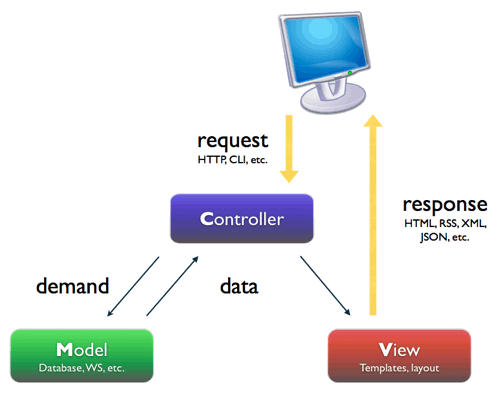
\includegraphics[width=0.8\textwidth]{mvc.png}
\end{center}
\begin{itemize}
  \item \textbf{Camada de Modelo} (Model) é a responsável pela interação com o banco de dados. 
  \item \textbf{Camada de Visão} (View) é a responsável por mostrar os dados na tela.
  \item \textbf{Camada de Controle} (Controller) é quem gerencia toda a comunicação entre uma Modelo e uma Visão. Não é permitido uma Visão acessar diretamente uma Modelo ou vice-versa.
\end{itemize}
Simplificadamente pense em uma empresa na qual existe um cliente que deseja falar com um determinado funcionário, porém para acessar sua sala deve passar por uma Secretária. Esse funcionário deseja obter uma determinada informação de um arquivo, para isso deve solicitá-la a Secretária. Ou seja, a Secretária é a controladora de tudo o que será permitido visualizar ou obter de informação da empresa.

\subsection{O que são Serviços}
A tecnologia de Serviços Web fornece uma série consideráveis benefícios para o desenvolvimento de aplicativos, uma vez que propicia a agilidade requerida pelas empresas frente às mudanças que podem ocorrer no ambiente de negócios. A grande vantagem no uso dos serviços Web provém da capacidade de permitir uma rápida e independente construção de várias 'Visões' de sistemas nas mais diversas plataformas existentes. 
\begin{center} 

\includegraphics[width=0.8\textwidth]{servicos.png}
\end{center}
Por exemplo, uma vez construída a camada de serviços, podemos utilizar o PhoneGap/Cordova para construir uma camada que será acessível pela plataforma Mobile, uma outra em Java/Swing para acessar via Desktop, uma terceira em Amber.js com um sistema Web, e todas utilizando a mesma camada de Serviço. \\[2mm]
Um Serviço Web é atualmente utilizado para integração entre aplicações. O Web Service REST é uma das formas de se criar um Serviço Web, que é utilizada com o protocolo HTTP. O conjunto de operações, suportadas pelo serviço, podem ser de quatro tipos: 
\begin{itemize}
  \item \textbf{GET}. Listar todos os membros dos recursos de coleção ou recuperar uma 
  determinada representação de um recurso identificado como 1234.
  \item \textbf{POST}. Criar um novo recurso na coleção em que o ID dele seja automaticamente designado ou obter todos os recursos de uma coleção com base em um filtro.
  \item \textbf{PUT}. Atualizar (substituir) determinados campos de um recurso identificado como 1234.
  \item \textbf{DELETE}. Eliminar uma coleção ou um determinado recurso identificado como 1234.
\end{itemize}
Serviços Web se consolidaram como uma base para disponibilização de negócios eletrônicos, dentre as quais se destacam organizações que atuam em diversos mercados, tais como Google, Amazon, GM, Fedex, Governo Federal. Isso permite a construção de uma rede intra/interorganizacional de aplicações colaborativas e distribuídas, onde os Serviços Web, na forma de módulos auto-contidos, são descritos, publicados, localizados e dinamicamente invocados através de camadas de diversas visões.

\section{Instalação do Sails.js}
Para proceder a instalação do Sails é necessário primeiro instalar o Node.js
que pode ser obtido em \url{https://nodejs.org/en/} e o NPM  em \url{https://www.npmjs.com/} \\[3mm]
Para instalar o Sails (lembrando que 'sudo' só necessário se estivermos em
ambiente Linux), em uma janela de comandos, digitar o seguinte: \\[1mm]
{\ttfamily\$ sudo npm install -g sails} \\[3mm]
Pronto, simples assim.

\subsection{Testar a instalação com um Projeto}
Para criar um projeto: \\[1mm]
{\ttfamily\$ sails new testProject --linker} \\[3mm]
A opção '--linker' faz com que quaisquer recursos sob a pasta /assets sejam copiados para a pasta .tmp/public pelo Grunt quando Sails for levantado. Uma das grandes vantagens do Sails é que também podemos criar o projeto apenas como um provedor de Serviços, isto é, sem a Camada de Visão, para isso utilizamos a seguinte opção: \\[1mm]
{\ttfamily\$ sails new myApi --no-frontend} \\[3mm]
O próximo passo é acessar a pasta: \\[1mm]
{\ttfamily\$ cd testProject} \\[3mm]
Disponibilizar o bower para o projeto, de modo a instalarmos novos componentes (responda todas as perguntas de forma adequada): \\[1mm]
{\ttfamily\$ bower init} \\[3mm]
Iniciar o sails: \\[1mm]
{\ttfamily\$ sails lift} \\[3mm]
Se tudo estiver funcionando corretamente é possível acessar o site de boas vindas no endereço: \\[1mm]
\url{http://localhost:1337/} \\[3mm]
Para interromper o servidor, realizar a seguinte sequencia {\ttfamily Ctrl+C} na janela de comandos.

\subsection{Geração dos Artefatos}
A maior vantagem em se utilizar o Sails é que este permite gerar as camadas MVC automaticamente, sem precisarmos perder tempo com configurações desnecessárias. A pasta /api contém todos os arquivos backend. A pasta /api/policies estão armazenadas regras para o acesso do usuário da aplicação. A pasta /api/responses contém arquivos como os erros do Servidor Web (404, 403, 500, entre outros). Adicionamos nessa pasta as funções que lidam com tarefas específicas, como decidir como gerenciar usuários com diferentes níveis de acesso. Poderia ser feito na Camada de Controle, mas não é uma boa prática controladores com um monte de lógica de negócios. \\[3mm]
As camadas MVC do projeto gerado podem ser encontradas nas seguintes pastas:
\begin{itemize}
  \item \textbf{Camada de Modelo} que está disponível na pasta /api/models do projeto gerado, arquivos no padrão .js
  \item \textbf{Camada de Controle} que está disponível na pasta /api/controllers do projeto gerado, arquivos no padrão .js
  \item \textbf{Camada de Visão} que está disponível na pasta /views do projeto gerado, arquivos no padrão .ejs 
  (esta camada não é gerada automaticamente)
\end{itemize}
Gerar a Model e a Controller: \\[1mm]
{\ttfamily\$ sails generate api |Nome|} \\[3mm]
Por exemplo: \\[1mm]
{\ttfamily\$ sails generate model Pet} \\[3mm]
Gerar a Controller: \\[1mm]
{\ttfamily\$ sails generate controller |Nome| |Ação|} \\[3mm]
Por exemplo: \\[1mm]
{\ttfamily\$ sails generate controller Artigo create find update destroy} \\[1mm]
{\ttfamily\$ sails generate controller Comentario create destroy tag like} \\[3mm]
Gerar a Model: \\[1mm]
{\ttfamily\$ sails generate model |Nome| |Attribute:Type|} \\[3mm]
Por exemplo: \\[1mm]
{\ttfamily\$ sails generate model Cliente nome:string endereco:string idade:integer}

\subsection{Um pequeno teste}
Vamos criar uma simples estrutura apenas para verificarmos se tudo está bem fixado até aqui. Criar um projeto conforme descrito e neste executar o seguinte comando: \\[1mm]
{\ttfamily\$ sails generate api teste} \\[3mm]
Dois arquivos foram criados, um na pasta '/api/models' chamado 'Teste.js' e outro na pasta '/api/controllers' chamado 'TesteController.js'. No primeiro arquivo modificar a codificação 
do modelo para:
\begin{lstlisting}
module.exports = {
  attributes: {
    value: {
      'nome': 'text'
    }
  }
};
\end{lstlisting}
E finalmente ativar o sails: \\[1mm]
{\ttfamily\$ sails lift} \\[3mm]
Agora será preciso utilizar um cliente para acessar os serviços expostos. Existem vários pessoalmente prefiro o 'Postman':
\begin{center} 
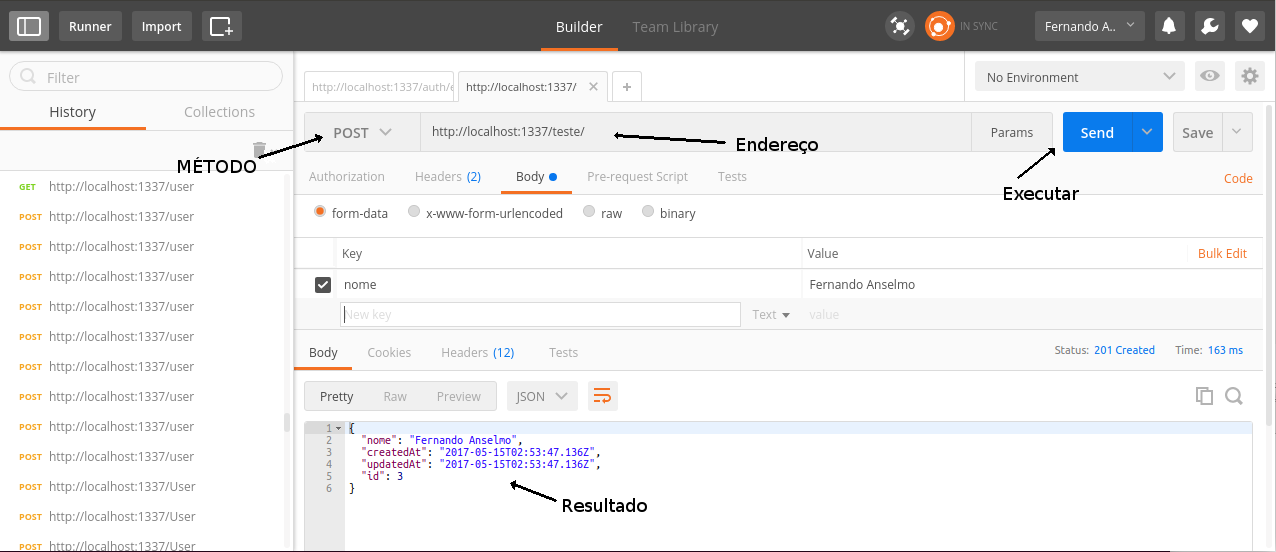
\includegraphics[width=0.8\textwidth]{Postman.png} 
\end{center}
E com ele, podemos acessar os seguintes serviços:
\begin{itemize}
  \item \textbf{http://localhost:1337/teste} método GET que traz todos os nomes cadastrados
  \item \textbf{http://localhost:1337/teste/1} método GET que traz o nome com o ID igual a 1
  \item \textbf{http://localhost:1337/teste} método POST que ao ser passado a variável nome no BODY de um formulário esta será armazenada no banco.
  \item \textbf{http://localhost:1337/teste/1} método UPDATE que ao ser passado a variável nome no BODY de um formulário esta será armazenada no banco no lugar do ID igual a 1 
  \item \textbf{http://localhost:1337/teste/1} método DELETE que irá excluir o ID com o valor igual a 1
\end{itemize}

\subsection{Arquivos de Configuração}
Outros arquivos importantes serão bastante utilizados são:
\begin{itemize}
  \item \textbf{/config/sockets.js}: este arquivo contém dois métodos, "onConnect" e "onDisconnect". Utilizamos este para proceder as conexões de socket.
  \item \textbf{/config/routes.js}: este arquivo nos permite a definição de URLs com as Visões e endpoints para os métodos da Camada de Controle.
  \item \textbf{/config/models.js}: este arquivo nos permite especificar os conectores para o Banco de Dados além de definir como migar os dados.
\end{itemize}
Por padrão o Sails acessa um ORM (Object Relational Mapper) chamado Waterline que podemos utilizar para realizar testes no sistema, não se preocupe pois é possível (através do uso de adaptadores) se conectar a, basicamente, todos os bancos conhecidos do mercado. \\[3mm]
No arquivo /config/models.js é possível definirmos o modo como a base de dados irá tratar os dados, são eles:
\begin{itemize}
  \item \textbf{safe}. Nunca migrar automaticamente a base de dados (usado por padrão, se nada for definido).
  \item \textbf{alter}. Migrar os dados, mas manter os dados já existentes (experimental).
  \item \textbf{drop}. Cada vez que o Servidor for reiniciado, eliminar TODOS os dados e reconstruir TODOS os modelos.
)
\end{itemize}
Também podemos subir o servidor com um dessas opções. Por exemplo: \\[1mm]
{\ttfamily\$ sails lift --models.migrate='alter'}
 
\subsection{Acessar o MySQL no Docker}
Antes de mais nada precisamos do banco MySQL rodando no Docker, para conseguir realizar isso assista o vídeo disponível no meu canal no endereço \url{https://www.youtube.com/watch?v=skx_Oxdw9i0&t=183s} e uma vez que o banco estiver configurado, acessar com o comando: \\[1mm]
{\ttfamily\$ docker exec -it mybanco mysql -p} \\[3mm]
Usar a senha 'root' para entrar e criar a base para este exemplo com o comando \\[1mm]
{\ttfamily create database demo;} \\[3mm]
Sair do MySQL com o comando: \\[1mm]
{\ttfamily exit} \\[3mm]
Criar um projeto para o Sails conforme descrito e neste executar o seguinte comando: \\[1mm]
{\ttfamily\$ sails generate api cliente} \\[3mm]
Modificar o arquivo 'connections.js' na pasta '/config' para a seguinte codificação:
\begin{lstlisting}
module.exports.connections = {
  localDiskDb: {
    adapter: 'sails-disk'
  },
  sailsmysql: {
    adapter: 'sails-mysql',
    host: '127.0.0.1',
    port: 3306,
    user: 'root',
    password: 'root',
    database: 'demo'
  }
};
\end{lstlisting}
Modificar o arquivo 'models.js' na pasta '/config' para a seguinte codificação:
\begin{lstlisting}
module.exports.models = {
  connection: 'sailsmysql',
  migrate: 'alter'
};
\end{lstlisting}
E o arquivo 'Cliente.js' na pasta '/api/models' para a seguinte codificação:
\begin{lstlisting}
module.exports = {
  attributes: {
    nome: {
      type: 'string',
      required: true
    },
    email: {
      type: 'email',
      required: true,
      unique: true
    }
  }
};
\end{lstlisting}
O último passo é adicionar a biblioteca de conexão com o MySQL com o seguinte comando: \\[1mm]
{\ttfamily\$ npm install sails-mysql --save} \\[3mm]
Executar o Sails: \\[1mm]
{\ttfamily\$ sails lift} \\[3mm]
E execute os seguintes comandos em um navegador (como complemento para \url{http://localhost:1337}):
\begin{itemize}
  \item \textbf{/cliente/create?nome=Fernando\&email=anselmo@gmail.com} \\
  cadastrar um novo cliente com o nome: 'Fernando' e email: 'anselmo@gmail.com'.
  \item \textbf{/cliente/update/1?nome=Fernando Anselmo} \\
  modificar o cliente com o ID igual a 1 para o nome: 'Fernando Anselmo'.
  \item \textbf{/cliente/destroy/1} \\
  eliminar o cliente com o ID igual a 1 do banco.
\end{itemize}
Observe que automaticamente o Sails cria no banco alguns campos como chave primária e datas de atualização, podemos não desejar que ele se comporte dessa forma para isso, no modelo, entre a instrução ``exports'' e ``atributes'' colocamos as seguintes instruções:
\begin{itemize}
  \item \textbf{autoCreateAt: false,}: para não criar a data de criação do registro
  \item \textbf{autoUpdateAt: false,}: para não criar a data de atualização do registro
  \item \textbf{autoPK: false,}: para não criar a chave primária  
\end{itemize}

\subsection{Ajuste da saída Dados}
Com o Sails podemos criar uma controller com dois passos simples (se a Model já tiver pronta então será apenas um passo) para nos devolver basicamente qualquer conjunto de dados que desejemos. Por exemplo uma nova saída com base em uma consulta SQL que agrupe os dados. Vamos aproveitar o projeto visto com o banco MySQL para realizar essa tarefa. Adicione uma nova Model e Controler com o seguinte comando: \\[1mm]
{\ttfamily\$ sails generate api Conta} \\[3mm]
Modificar o arquivo 'Conta.js' na pasta '/api/models' para a seguinte codificação:
\begin{lstlisting}
module.exports = {
  attributes: {
    dtEntrada: {
      type: 'datetime',
      required: true
    },
    valor: {
      type: 'float',
      required: true
    }
  }
};
\end{lstlisting}
Crie a maior quantidade de dados que desejar variando as informações de ``data de entrada'' e ``valor'' o máximo possível. O segundo passo é adicionar um novo método de chamada no arquivo 'ContaController.js' na pasta '/api/controllers' com a seguinte codificação:
\begin{lstlisting}
module.exports = {
  graph2: function (req, res) {
    var myQuery = "select month(dtEntrada) as mes, sum(valor) as valor from conta " +
 		  "group by month(dtEntrada)";
    var meses = [];
    var valor = [];
    Conta.query(myQuery, function (err, contas){
    if (err) {
      return res.json({"status": 0, "error": err});
    } else {
      for (var key in contas) {
	if (contas.hasOwnProperty(key)) {
	  meses.push(contas[key].mes);
	  valor.push(contas[key].valor);
	}
      }
    return res.json({"mes": meses, "valor": valor});
    }
  });
}
\end{lstlisting}
Selecionamos da base de dados, mês a mês o somatório dos valores e montamos para a saída um JSON com dois arrays ``mes'' e ``valor'', é ideal para carregar uma visão com o \textbf{Chart.js} com a montagem de um gráfico.

\subsection{Adicionar o Bootstrap e a JQuery ao projeto}
O Bootstrap e a JQuery consolidaram-se como padrões de mercado, para disponibilizá-los em nosso projeto devemos seguir os seguintes passos: \\[3mm]
1. Criar na raiz do projeto um arquivo chamado .bowerrc com o seguinte conteúdo: \\[1mm]
\textbraceleft {\ttfamily ``directory'' : ``assets/vendor''} \textbraceright \\[3mm]
2. Instalar o Bootstrap com o comando (é instalada a JQuery automaticamente): \\[1mm]
{\ttfamily\$ bower install bootstrap --save --production} \\[3mm]
3. Adicionar a linha no arquivo /assets/styles/importer.less: \\[1mm]
{\ttfamily @import '../vendor/bootstrap/less/bootstrap.less';} \\[3mm]
4. Copiar a pasta /assets/vendor/bootstrap/fonts embaixo da pasta /assets. \\[3mm]
5. Adicionar os seguintes comandos no arquivo /tasks/pipeline.js, após a instrução 'sails.io.js':
\begin{lstlisting}
'js/dependencies/sails.io.js',
// Adicionar a JQuery JS
'vendor/jquery/dist/jquery.min.js',
// Adicionar o Bootstrap JS
'vendor/bootstrap/dist/js/bootstrap.min.js',
\end{lstlisting}
Agora o projeto conta com o poder do Bootstrap e da JQuery.

\subsection{Mais um teste da Instalação}
Iremos realizar um exemplo mais completo para verificar se tudo está funcionando corretamente. Na pasta /views, no arquivo 'layout.ejs', localizar a linha com a instrução '\textless\%- body \%\textgreater' e alterar para:
\begin{lstlisting}
    <nav class="navbar navbar-inverse navbar-fixed-top">
      <div class="container">
        <div class="navbar-header">
          <button type="button" class="navbar-toggle collapsed" data-toggle="collapse" data-target="#navbar" aria-expanded="false" aria-controls="navbar">
            <span class="sr-only">Toggle navigation</span>
            <span class="icon-bar"></span>
            <span class="icon-bar"></span>
            <span class="icon-bar"></span>
          </button>
          <a class="navbar-brand" href="/">Sails Exemplo</a>
        </div>
        <div id="navbar" class="navbar-collapse collapse">
          <form class="navbar-form navbar-right">
            <div class="form-group">
              <input type="text" placeholder="Email" class="form-control">
            </div>
            <div class="form-group">
              <input type="password" placeholder="Senha" class="form-control">
            </div>
            <button type="submit" class="btn btn-success">Entrar</button>
          </form>
        </div><!--/.navbar-collapse -->
      </div>
    </nav>
    <%- body %>
    <div class="container">
      <hr />
      <footer class="footer">
        <div class="pull-right">
          <a href="http://sailsjs.com">sails.js</a>
          <div>Construído com o Sails</div>
        </div>
      </footer>
    </div>  
\end{lstlisting}
Definimos aqui um cabeçalho e rodapé padrão para todas as páginas do projeto. Criar uma nova pasta abaixo dessa pasta chamada '/static' e nesta criar um arquivo chamado 'index.ejs' com o seguinte conteúdo:
\begin{lstlisting}
<div class="jumbotron">
  <div class="container">
    <h2>Exemplo do Sails com Bootstrap e JQuery</h2>
    <p>Verificar se tudo está funcionando corretamente...</p>
  </div>
</div>
\end{lstlisting}
Modificar a rota padrão, no arquivo de rotas (/config/routes.js), para:
\begin{lstlisting}
  '/': {
    view: 'static/index'
  }
\end{lstlisting}
E ao levantar o Sails teremos o seguinte resultado na página inicial:
\begin{center} 
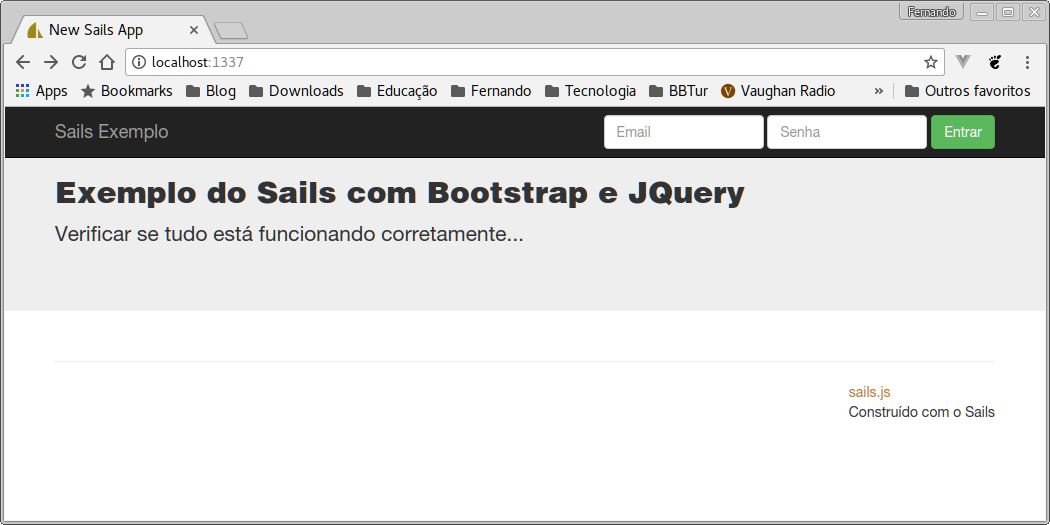
\includegraphics[width=0.8\textwidth]{sailsEx01.png}
\end{center}

\section{Modelagem de Dados}
Agora que sabemos como instalar, criar e configurar corretamente um projeto no
Sails. Vamos criar um exemplo para testar um modelo de dados como forma de conhecer melhor suas potencialidades.
\begin{center} 

\includegraphics[width=0.8\textwidth]{hero_squid.png} 
\end{center}
A empresa MeuPet deseja melhorar os serviços de implantação de sua intranet 
com buscas no aprimoramento de disponibilização de serviços. A estrutura da 
base de dados foi definida através do rascunho das seguintes tabelas: \\[3mm]
{\ttfamily Cliente}
\begin{itemize}
  \item \textbf{priNome}. String (obrigatório), primeiro nome
  \item \textbf{ultNome}. String (obrigatório), último nome
  \item \textbf{endereco}.  Text, endereço de residência
  \item \textbf{email}. String (válido), endereço eletrônico de contato
  \item \textbf{telefone}. String (obrigatório), número do telefone de contato
\end{itemize}
{\ttfamily Pet}
\begin{itemize}
  \item \textbf{idDono}. String (obrigatório), campo de associação com o cliente
  \item \textbf{genero}. String, gênero do animal que só deve permitir: 'Macho' ou 'Fêmea'
  \item \textbf{datNascimento}. Date, contendo a data nascimento
  \item \textbf{especie}. String, espécie do animal que só deve permitir: 'Cachorro' ou 'Gato'
  \item \textbf{raca}. String, descricao da raça do animal
  \item \textbf{caracteristica}. Text, campo livre para observações sobre o animal
\end{itemize}
{\ttfamily Servico}
\begin{itemize}
  \item \textbf{inicial}. Date, data e hora inicial do serviço
  \item \textbf{idpet}. String (obrigatório), campo de associação com o animal
  \item \textbf{tipo}. String, tipo do serviço que só deve permitir: 'Consulta', 'Banho' ou 'Tosa'
  \item \textbf{descricao}. Text, descrição completa do serviço a ser realizado
  \item \textbf{status}. String, situação do serviço que só deve permitir: 'Agendado' ou 'Finalizado'
  \item \textbf{buscar}. Boolean, se é ou não para buscar o animal
  \item \textbf{levar}. Boolean, se é ou não para levar o animal ao término do serviço
\end{itemize}
Todas as tabelas possuem dois campos obrigatórios que não são informados no cadastro:
\begin{itemize}
  \item \textbf{id}. String, chave única
  \item \textbf{adicionadoEm}. Date, contendo a data de cadastro
\end{itemize}

\subsection{Implementando para o Banco de Dados}
Como banco de dados usaremos o RethinkDB, um banco de dados ORM, open-source, escalável com foco na criação de aplicativos em tempo real mais fácil. Qual a diferença para o MongoDB? Um gerenciador que nos permite controla visualmente o banco, ou seja, temos uma maior capacidade administrativa, mas não se preocupe esse projeto pode ser adaptado para qualquer banco que deseje. \\[3mm]
Para instalar o banco usaremo uma imagem do Docker, então com o Docker já instalado podemos digitar simplesmente o seguinte comando para baixarmos a imagem oficial: \\[1mm]
{\ttfamily\$ docker pull rethinkdb} \\[3mm]
E o seguinte comando para rodá-la e ativar o banco: \\[1mm]
{\ttfamily\$ docker run -d -p 8080:8080 -p 28015:28015 -p 29015:29015 --name } \\[1mm]
{\ttfamily rethink1 rethinkdb} \\[3mm]
O banco está ativo na porta 28015, a porta 29015 é de controle do RethinkDB e a porta
8080 é sua parte administrativa, abra um navegador e acesse o endereço 
\url{http://localhost:8080} e veremos a seguinte imagem:
\begin{center} 
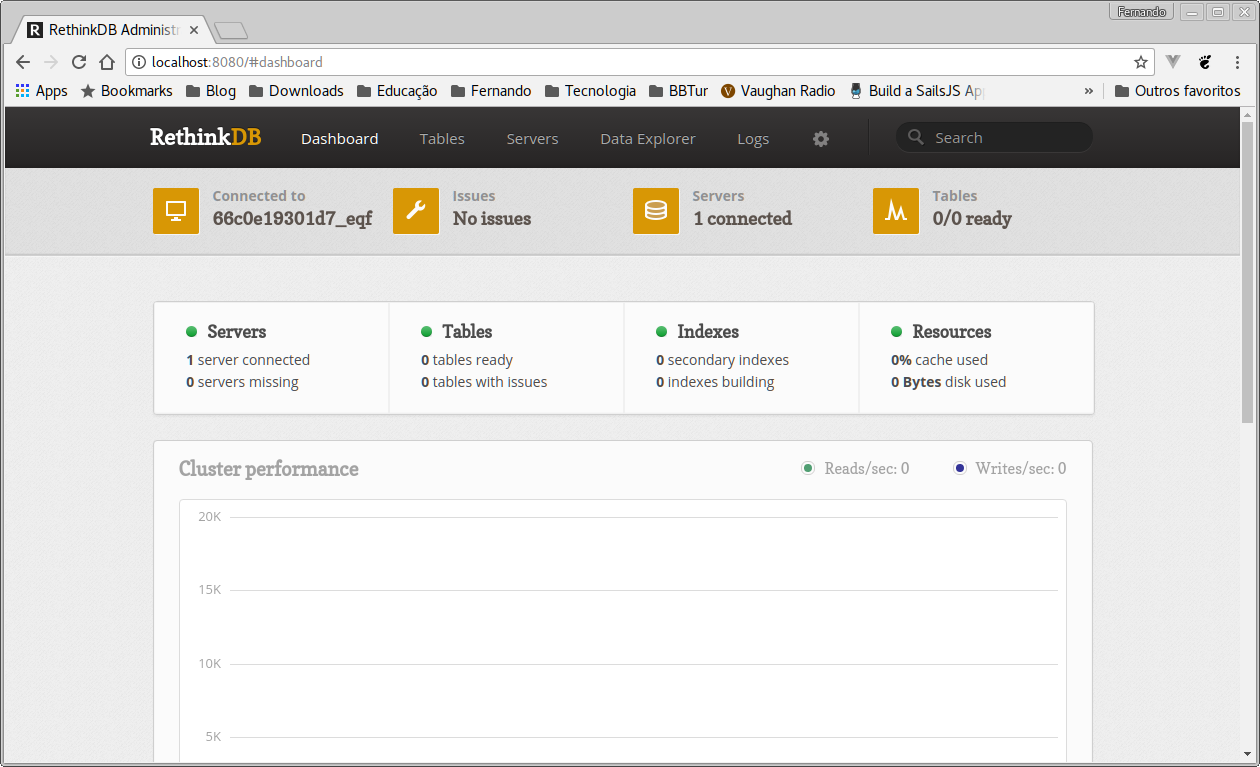
\includegraphics[width=0.8\textwidth]{Rethinkdb.png} 
\end{center}
Se deseja parar o banco de dados basta digitar o seguinte comando: \\[1mm]
{\ttfamily\$ docker stop rethink1} \\[3mm]
E para ativá-lo novamente: \\[1mm]
{\ttfamily\$ docker start rethink1}

\subsection{Configurar o Banco de Dados}
Na pasta do projeto, adicionar os seguintes módulos necessários para realizar a conexão com o banco: \\[1mm]
{\ttfamily\$ npm install thinky thinky-loader --save} \\[3mm]
No arquivo 'package.json' adicione a seguinte linha na seção 'dependencies': \\[1mm]
{\ttfamily "sails-rethinkdb": "github:gutenye/sails-rethinkdb\#master",} \\[3mm]
E instale esta dependência: \\[1mm]
{\ttfamily\$ npm install} \\[3mm]
Após a instalação corrigir um erro que cria tabelas duplicadas, editar a classe 'connection.js' na pasta /node\_modules/sails-rethinkdb/lib e comentar as seguintes instruções na função \_setupTables(tables):
\begin{lstlisting}
  this.db.tableCreate(name).run(this.conn, err => {
    if (err && !err.message.match(/Table `.*` already exists/))
      throw err
  })
\end{lstlisting}
Com essa primeira parte pronta vamos realizar as seguintes modificações nos arquivos do projeto. No arquivo 'config/connections.js' adicionar a seguinte instrução (abaixo da expressão de 'localDiskDb'):
\begin{lstlisting}
  rethinkdb: {
    adapter: 'sails-rethinkdb',
    host: 'localhost',
    db: 'petshop'
  }
\end{lstlisting}
Criar uma pasta chamada '/hooks' abaixo da pasta '/api'. Nesta pasta criar um arquivo chamado 'thinkhook.js', com as seguintes instruções:
\begin{lstlisting}
module.exports = function(sails){
  return {
    connecting: function () {
      let orm = require('thinky-loader');
      let path = require('path');
      var dir = path.resolve(__dirname, '../models');
      let ormConfig = {
        debug     : true, 
        modelsPath: dir,
        thinky    : {
          rethinkdb: {
            host        : 'localhost',
            port        : 28015,
            authKey     : '',
            db          : 'petshop',
            timeoutError: 5000,
            buffer      : 5,
            max         : 1000,
            timeoutGb   : 60 * 60 * 1000
          }
        }
      };
      orm.initialize(ormConfig)
      .then(() => console.log('RethinkDB está pronto para uso!'))
      .catch((e) => console.log(e));
    },
    initialize: function (cb) {
      this.connecting();
      sails.emit('hook:thinkhook:done');
      return cb();
    },
  }
}  
\end{lstlisting}
Na inicialização também é possível passar o comando 'orm.initialize(ormConfig, thinky)' que repassa uma instância do thinky para uma configuração adicional. Nosso próximo passo é modificar o arquivo '/config/models.js':
\begin{lstlisting}
module.exports.models = {
  connection: 'rethinkdb',
  migrate: 'safe'
};  
\end{lstlisting}
Se tudo está funcionando corretamente, ao reiniciar o servidor é recebida a seguinte mensagem: \\[3mm]
{\ttfamily Creating a pool connected to localhost:28015} \\[1mm]
{\ttfamily RethinkDB está pronto para uso!} \\[1mm]
Além disso no Administrador do RethinkDB, na seção Tables, é mostrada a base de 
dados 'petshop'.

\subsection{Criação dos Modelos e Controles}
Começaremos criando os três modelos/controles necessários: \\[3mm]
{\ttfamily\$ sails generate api Cliente} \\[1mm]
{\ttfamily\$ sails generate api Pet} \\[1mm]
{\ttfamily\$ sails generate api Servico} \\[3mm]
Agora vamos alterar cada uma dos modelos (na pasta /api/models) para criar
corretamente a estrutura das nossas tabelas conforme definido. \\[3mm]
{\ttfamily Arquivo: Cliente.js}
\begin{lstlisting}
 module.exports = function() {
   let thinky = this.thinky;
   let validator = require('validator');
   let type = this.thinky.type;
   let models = this.models;
   return {
     tableName: 'cliente',
     schema: {
       id: type.string(),
       priNome: type.string().required(),
       ultNome: type.string().required(),
       endereco: type.string(),
       email: type.string().validator(validator.isEmail),
       telefone: type.string().required(),
       adicionadoEm: type.date().default(new Date())
     },
     options: {},
     init: function(model) { }
   };
 };
 \end{lstlisting}
{\ttfamily Arquivo: Pet.js}
\begin{lstlisting}
module.exports = function() {
  let thinky = this.thinky;
  let validator = require('validator');
  let type = this.thinky.type;
  let models = this.models;
  return {
    tableName: 'pet',
    schema: {
      id: type.string(),
      idDono: type.string().required(),
      genero: type.string().enum("Macho", "Fêmea"),
      datNascimento: type.date(),
      especie: type.string().enum("Cachorro", "Gato"),
      raca: type.string(),
      caracteristica: type.string().required(),
      adicionadoEm: type.date().default(new Date())
    },
    options: {},
    init: function(model) {
      model.belongsTo(models.cliente, "dono", "idDono", "id");
    }
  };
};
\end{lstlisting}
{\ttfamily Arquivo: Servico.js}
\begin{lstlisting}
module.exports = function() {
  let thinky = this.thinky;
  let validator = require('validator');
  let type = this.thinky.type;
  let models = this.models;
  return {
    tableName: 'servico',
    schema: {
      id: type.string(),
      inicial: type.date().required(),
      idPet: type.string().required(),
      tipo: type.string().enum("Consulta", "Banho", "Tosa"),
      descricao: type.string(),
      status: type.string().enum("Agendado", "Finalizado"),
      buscar: type.boolean().default(false),
      levar: type.boolean().default(false),
      adicionadoEm: type.date().default(new Date())
    },
    options: {},
    init: function(model) {
      model.belongsTo(models.pet, "animal", "idPet", "id");
    }
  };
};
\end{lstlisting}
Se tudo está funcionando corretamente ao reiniciar o servidor é mostrada as mensagens de criação e inicialização das tabelas. Além disso no Administrador do RethinkDB, na seção Tables veremos na base de dados 'petshop' com as tabelas criadas conforme a seguinte imagem:
\begin{center} 
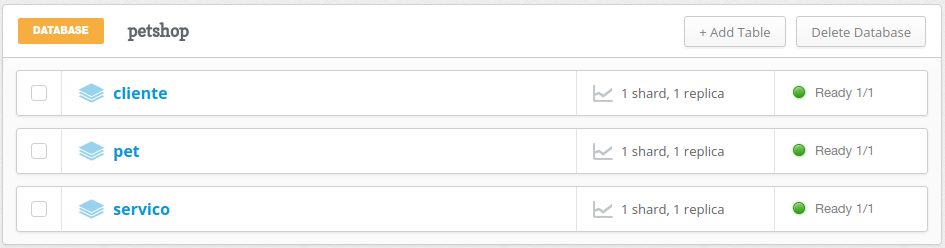
\includegraphics[width=0.8\textwidth]{tabelas.png} 
\end{center}
Se desejar um teste mais completo pode usar um aplicativo como o 'Postman' (ou outro aplicativo similar) para acessar os serviços que já estão criados, para cada tabela existe um CRUD completo pronto e funcionando, com métodos: GET, POST, PUT e DELETE.

\section{Conclusão}
Sails é um framework JavaScript que facilita a criação de aplicativos com o servidor Node.js a nível empresarial fornece um monte de recursos poderosos por padrão, para que possamos começar a desenvolver um aplicativo sem ter que pensar sobre a configuração. Foi projetado com base no conhecido padrão MVC e com um suporte aos requisitos de aplicativos modernos: APIs orientadas a dados com uma arquitetura escalonável orientada a serviços. É possível usá-lo para qualquer projeto de aplicativo da Web. \\[3mm]
Um desenvolvedor que possua experiência com aplicações frontend e está procurando um servidor ágil de JavaScript, pode encontrar no Sails uma boa solução. Este atende também aos que possuem experiência com aplicações backend em um idioma diferente de JavaScript e está procurando expandir seus conhecimentos em Node.js. Em ambos os casos, a familiaridade com Serviços Web pode ser o quisito mais importante sobre como construir uma aplicação web. \\[3mm]
Um conjunto de pequenos módulos trabalham em conjunto com o Sails para fornecer simplicidade, facilidade de manutenção e convenções estruturais aos aplicativos Node.js. Além disso o Sails é altamente configurável, assim não seremos forçados a manter toda uma funcionalidade que não é necessária para o projeto. Sou um entusiasta do mundo Open Source e novas tecnologias. Veja outros artigos que publico sobre tecnologia acessando meu Blog Oficial \cite{fernandoanselmo}.

%-----------------------------------------------------------------------------
% REFERÊNCIAS
%-----------------------------------------------------------------------------

\begin{thebibliography}{5}

  \bibitem{sailsoficial} 
  Página do Sails.js \\
  \url{http://sailsjs.com/}

  \bibitem{fernandoanselmo} 
  Fernando Anselmo - Blog Oficial de Tecnologia \\
  \url{http://www.fernandoanselmo.blogspot.com.br/}

  \bibitem{bootstrapoficial} 
  Página do Bootstrap \\
  \url{http://getbootstrap.com/}

  \bibitem{jqueryoficial} 
  Página da JQuery \\
  \url{https://jquery.com/}

  \bibitem{rethinkdboficial} 
  Página do RethinkDB \\
  \url{https://www.rethinkdb.com/}

\end{thebibliography}
  
\end{document}
